% One possible first three generations of the 0-or-2 offspring model.
% Every full node has either zero or two children. Drawn as a possible sample,
% not as a measured frequency or a probability mass.
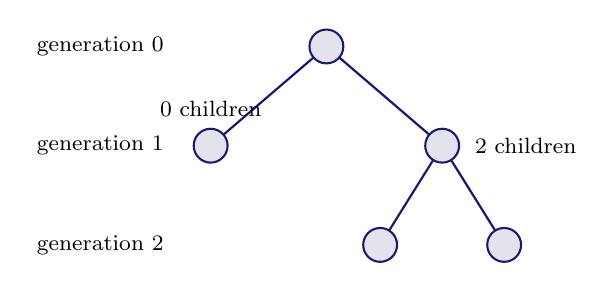
\begin{tikzpicture}[x=1.05cm,y=1.05cm,line cap=round]
  \tikzset{person/.style={circle,draw=MidnightBlue,fill=MidnightBlue!12,
                     line width=0.75pt,minimum size=0.43cm,inner sep=0pt}}
  \draw[MidnightBlue,thick] (0,2.4)--(-1.4,1.2) (0,2.4)--(1.4,1.2)
    (1.4,1.2)--(0.65,0) (1.4,1.2)--(2.15,0);
  \node[person] at (0,2.4) {};
  \node[person] at (-1.4,1.2) {};
  \node[person] at (1.4,1.2) {};
  \node[person] at (0.65,0) {};
  \node[person] at (2.15,0) {};
  \node[font=\footnotesize,anchor=east] at (-1.85,2.4) {generation $0$};
  \node[font=\footnotesize,anchor=east] at (-1.85,1.2) {generation $1$};
  \node[font=\footnotesize,anchor=east] at (-1.85,0) {generation $2$};
  \node[font=\footnotesize,anchor=south] at (-1.4,1.43) {$0$ children};
  \node[font=\footnotesize,anchor=west] at (1.68,1.2) {$2$ children};
\end{tikzpicture}
